\section{Instalación con Windows}
A continuación se muestra proceso de instalación en una edición Pro del Sistema Operativo Windows (Windows 10 Pro).

	\subsection{Verificación de software instalado previamente}
	se revisó la sección “Programas y características” de Windows con el propósito de identificar instalaciones existentes de Oracle Database que pudieran generar conflictos. No se encontraron instalaciones de Oracle Database XE ni Oracle Database; únicamente se identificaron Java 8 y Oracle VirtualBox.
	
		\begin{figure}[htbp]
			\centering
			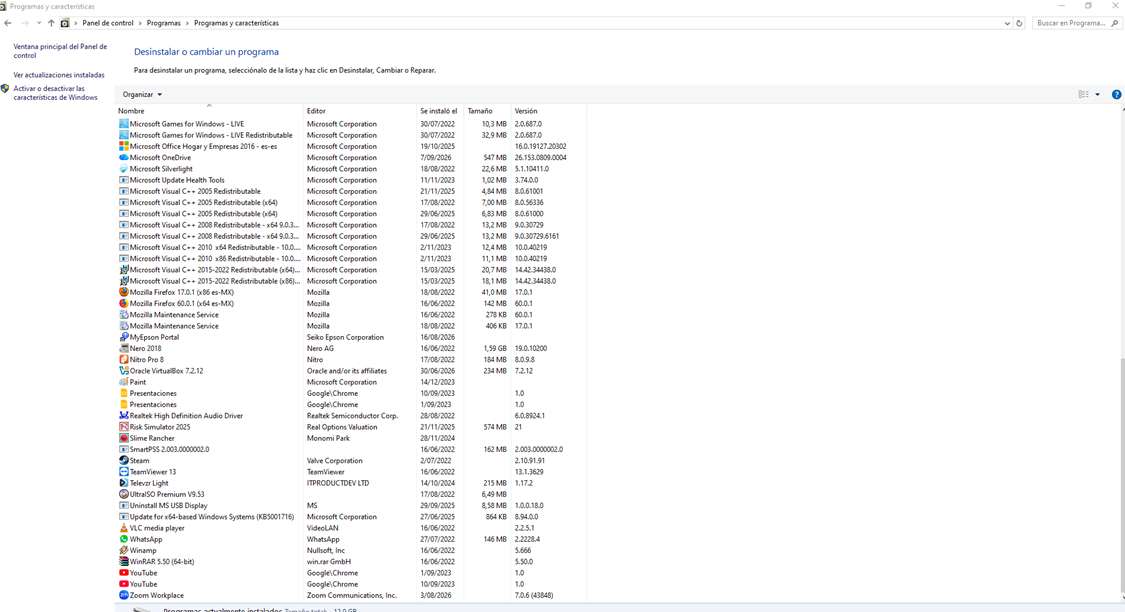
\includegraphics[width=1.0\textwidth]{../../images/w10pro01.png}
			\caption{Verificación de programas instalados}
			\label{fig:Verificación de programas instalados}
		\end{figure}
		\FloatBarrier
		
	\subsection{Descarga del instalador}
	En la página del instalador elegimos la opción para windows
		\begin{figure}[htbp]
			\centering
			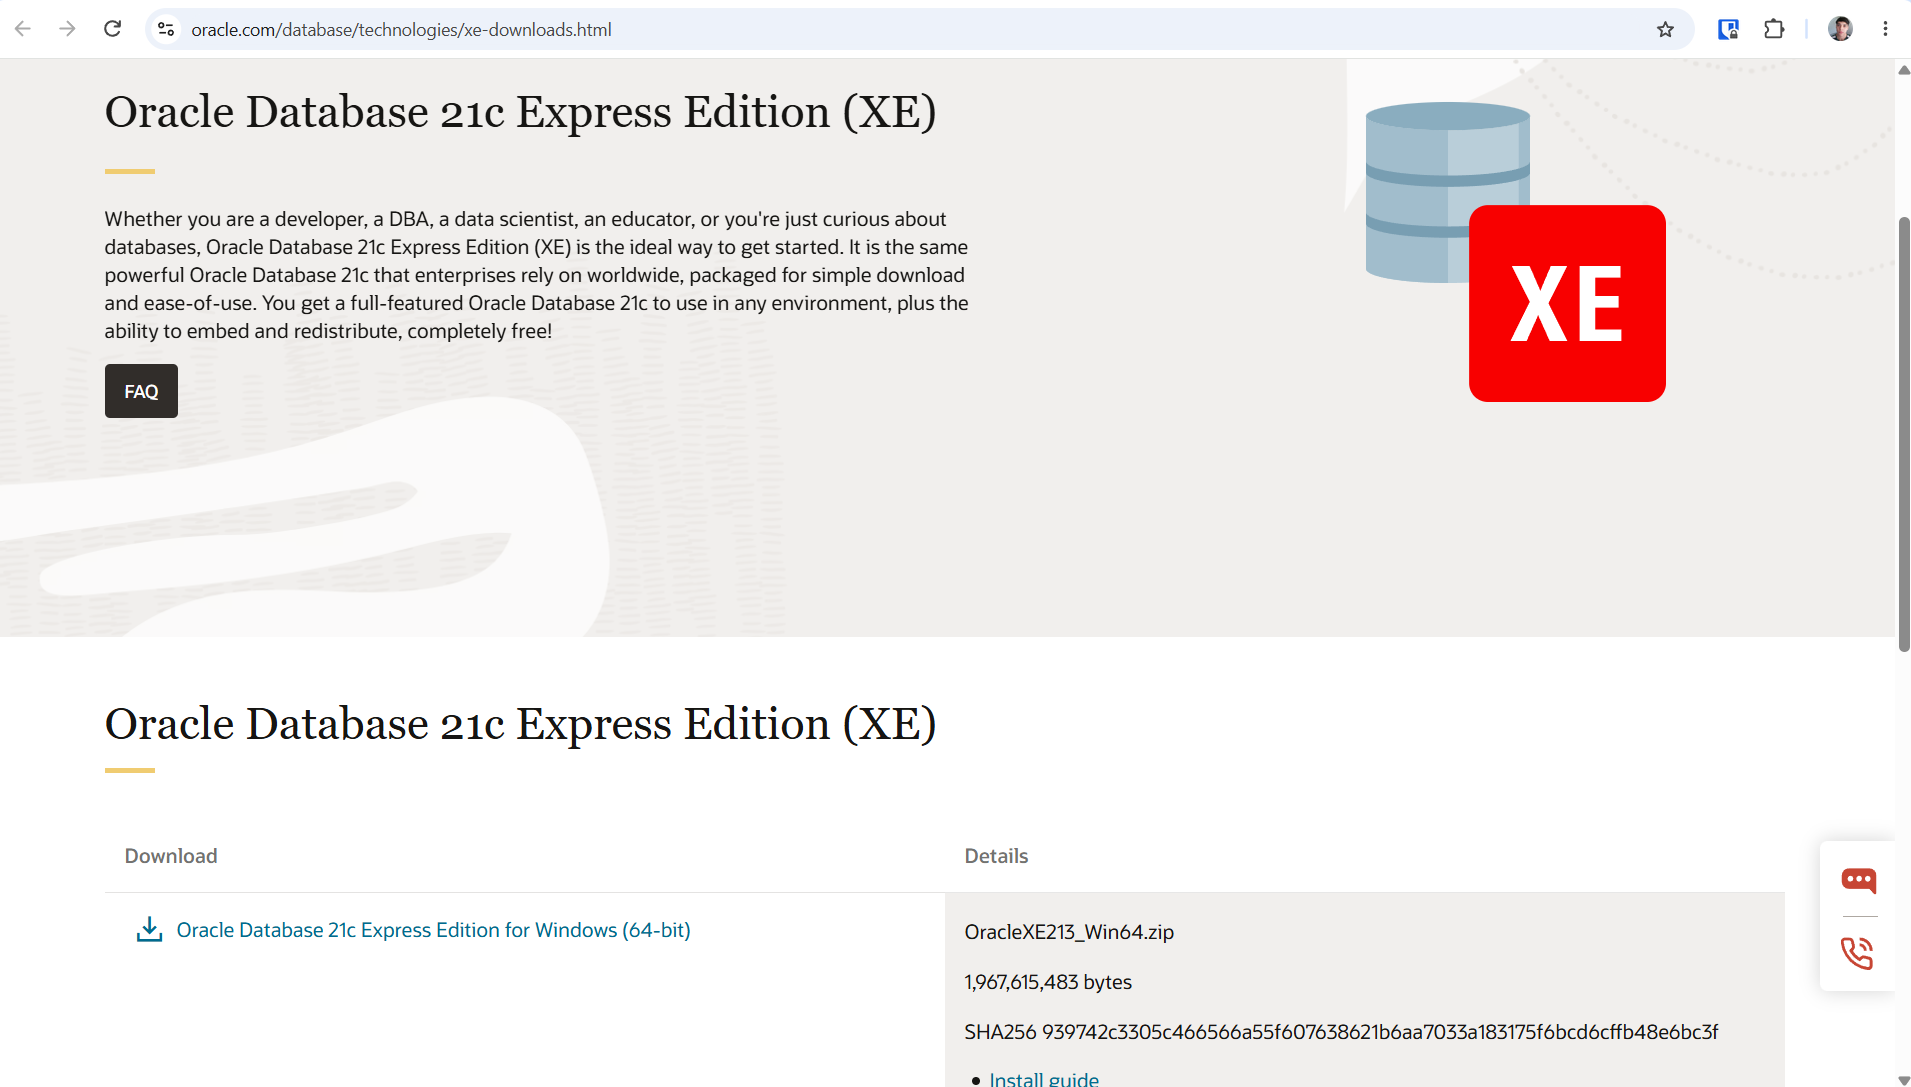
\includegraphics[width=1.0\textwidth]{../../images/w10pro02.png}
			\caption{Página oficial de descarga}
			\label{fig:Página oficial de descarga}
		\end{figure}
		\FloatBarrier
	
	\subsection{Descompresión del instalador y ejecución}
	Se debe descomprimir el .zip descargado y una vez terminada la descompresión ejecutar \textbf{setup.exe}, se abrirá el asistente de instalación al cuál se deberá dar click en siguiente, aceptar los términos del acuerdo de licencia, seleccionar directorio de destino (si en alguna porción de la ruta hay caracteres no permitidos deben borrarse, como por ejemplo los espacios), definir contraseña, dar clic en instalar, permitir acceso a redes públicas cuando se despliegue la pantalla del Firewall de Windows y esperar a que se complete la instalación.
	
	Para ver los pasos detallados del proceso ingresar al siguiente enlace:
	
	\vspace{0.5cm}
	\begin{center}
		\href{https://github.com/jota2209/GA4-210602033-AA1-EV02/blob/main/README.md}{→ Click aquí para instrucciones de instalación ←}
		
	\end{center}
	\vspace{0.5cm}
	
	